% Created 2021-02-24 mié 13:04
% Intended LaTeX compiler: pdflatex
\documentclass[presentation,aspectratio=169]{beamer}
\usepackage[utf8]{inputenc}
\usepackage[T1]{fontenc}
\usepackage{graphicx}
\usepackage{grffile}
\usepackage{longtable}
\usepackage{wrapfig}
\usepackage{rotating}
\usepackage[normalem]{ulem}
\usepackage{amsmath}
\usepackage{textcomp}
\usepackage{amssymb}
\usepackage{capt-of}
\usepackage{hyperref}
\usepackage{khpreamble}
\usepackage{amssymb}
\usepgfplotslibrary{groupplots}
\newcommand*{\shift}{\operatorname{q}}
\usetheme{default}
\author{Kjartan Halvorsen}
\date{2021-02-25}
\title{Retroalimentación Actividad 2 - Sistema sensorial}
\hypersetup{
 pdfauthor={Kjartan Halvorsen},
 pdftitle={Retroalimentación Actividad 2 - Sistema sensorial},
 pdfkeywords={},
 pdfsubject={},
 pdfcreator={Emacs 26.3 (Org mode 9.4.4)}, 
 pdflang={English}}
\begin{document}

\maketitle

\section{Sistemas mecatrónicos}
\label{sec:orgf9bc056}

\begin{frame}[label={sec:org1c8b699}]{Actividad 2}
\begin{block}{Propósito}
\begin{enumerate}
\item Identificar cuales serían \alert{las variables físicas más relevantes para un mejor control} del proceso y en base a esto \alert{definir las métricas funcionales} que debe cumplir el sistema sensorial.

\item Seleccionar un conjunto de \alert{equipos que cumpla con los requerimientos establecidos}, además de observar los aspectos económicos y de seguridad.
\end{enumerate}
\end{block}
\end{frame}

\begin{frame}[label={sec:orgc50fc9f}]{Análisis de un sistema mecatrónico}
\begin{block}{Requisitos / criterios de diseño}
\end{block}

\begin{block}{Identificar y describir elementos del sistem}
\begin{itemize}
\item mecanismo
\item actuadores
\item sensores
\item sistema de control
\end{itemize}
\end{block}
\end{frame}

\begin{frame}[label={sec:orgd970100}]{Requisitos / criterios de diseño}
 \begin{center}
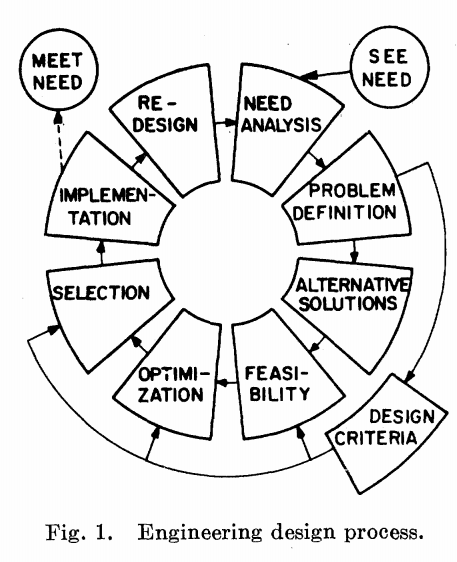
\includegraphics[height=0.6\textheight]{../../figures/design-process-fig1.png}\\
{\footnotesize  S.F. Love (1969) Modern design methods for electronics,  IEEE tr systems science and cybernetics}
\end{center}
\end{frame}


\begin{frame}[label={sec:orge425b73}]{Estudiantes contra expertos}
\begin{center}
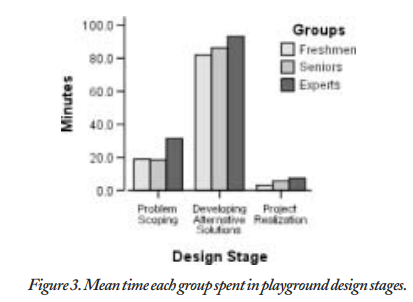
\includegraphics[width=0.5\linewidth]{../../figures/playground-design-student-experts.png}
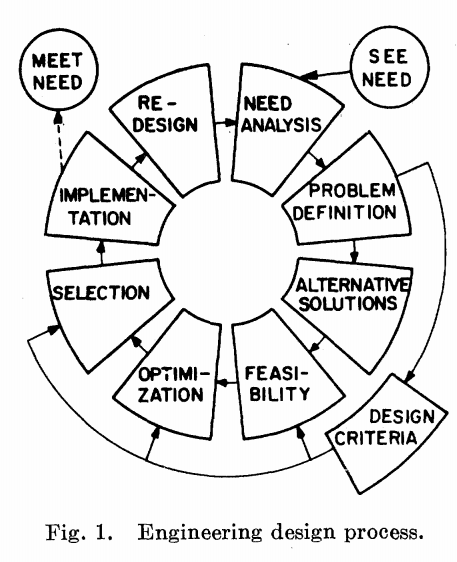
\includegraphics[width=0.3\linewidth]{../../figures/design-process-fig1.png}
\end{center}
\footnotesize Fig 3 de Atman et al. Engineering design processes: A comparison of students and expert practitioners. Journal of engineering education, 2007.
\end{frame}


\begin{frame}[label={sec:org89022f8}]{Sistema mecatrónico del AC75}
\begin{center}
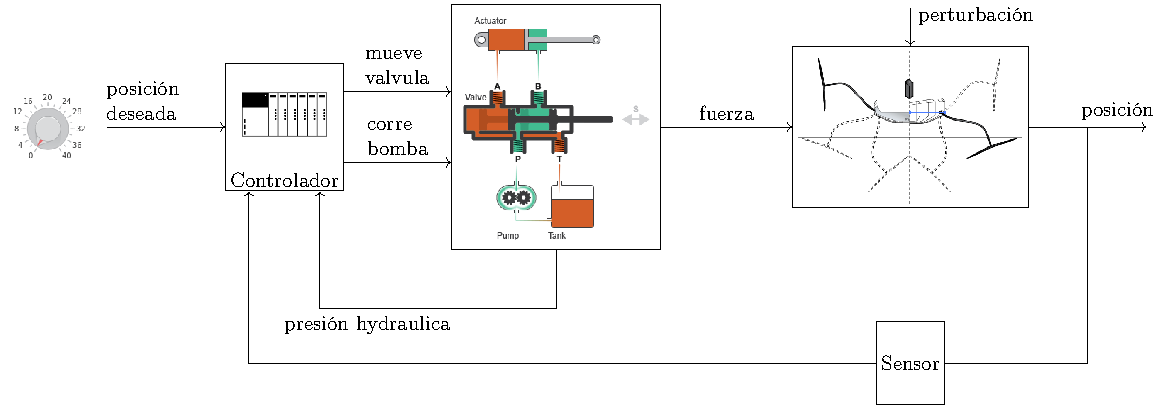
\includegraphics[width=.76\textwidth]{../../figures/ac75-control-block-details}
\end{center}

\begin{itemize}
\item \alert{Proceso} Aquí es un \alert{sistema mecanico} o \alert{mecanismo}
\item \alert{Actuador} Conversión de una señal de información a fuerza/torque/flujo/energía
\item \alert{Sensores}  Conversión de una variable física a una señal de información
\item \alert{Controlador} Computadora o microcontrolador o PLC, recibe señales, ejecuta el algoritmo de control, manda acción de control (señales) a los actuadores.
\end{itemize}
\end{frame}


\begin{frame}[label={sec:org55fb2de}]{Variables físicas}
\begin{columns}
\begin{column}{0.5\columnwidth}
\begin{center}
\includegraphics[height=0.8\textheight]{../../figures/ac75-class-foil.png}
\end{center}

{\footnotesize from the ac75 class rule}
\end{column}
\begin{column}{0.5\columnwidth}
\begin{center}
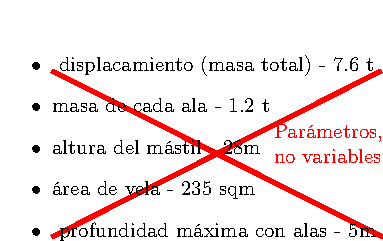
\includegraphics[width=0.8\textwidth]{../../figures/parameters-not-variables}
\end{center}
\end{column}
\end{columns}
\end{frame}

\begin{frame}[label={sec:orgb9d857c}]{Variables físicas}
\begin{columns}
\begin{column}{0.5\columnwidth}
\begin{center}
\includegraphics[height=0.8\textheight]{../../figures/ac75-class-foil.png}
\end{center}

{\footnotesize from the ac75 class rule}
\end{column}
\begin{column}{0.5\columnwidth}
\begin{itemize}
\item Posición angular continua del brazo/ala
\item Presión hydraulica
\item Estado de cargo de las pilas
\end{itemize}
\end{column}
\end{columns}
\end{frame}


\begin{frame}[label={sec:org9174ccf}]{Posición del ala - Requisitos}
\begin{columns}
\begin{column}{0.5\columnwidth}
\begin{center}
\includegraphics[height=0.6\textheight]{../../figures/ac75-class-foil.png}\\[-4mm]
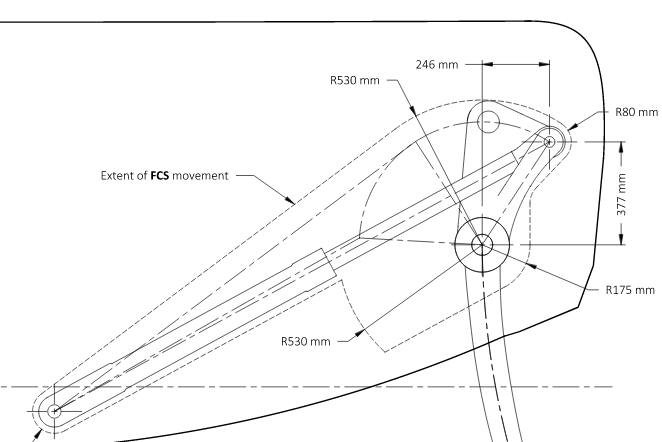
\includegraphics[height=0.3\textheight]{../../figures/ac75-rule-detail.png}
\end{center}
\end{column}

\begin{column}{0.5\columnwidth}
\begin{block}{Rango}
Gira de \(0^\circ\) (posición más abajo) hasta \(110^\circ\) (ala más arriba).
\end{block}

\begin{block}{Resolución}
Asumiendo resolución deseada de \(\epsilon_a = \unit{5}{\milli\meter}\) en la posición de la ala.

\begin{block}{En posición angular del brazo}
\(\epsilon_b = \frac{\epsilon_a}{r} = \unit{\frac{5}{3500}}{\rad} = \unit{0.08}{\degree}\)
\end{block}
\begin{block}{En posición lineal del pistón hidraulico}
\[ \epsilon_p = \unit{?}{\milli\meter}\]
\end{block}
\end{block}
\end{column}
\end{columns}
\end{frame}

\begin{frame}[label={sec:org43f076f}]{Posición del ala - Alternativ comercial 1}
\begin{center}
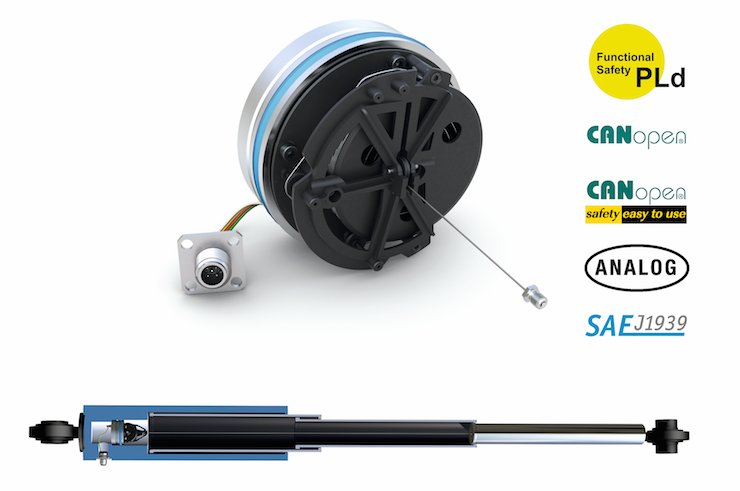
\includegraphics[width=0.3\linewidth]{../../figures/PosSensor.png}\\
{\footnotesize Fuente: SIKO GmbH}
\end{center}

\begin{center}
\begin{tabular}{lrlr}
Modelo & Rango [mm] & Resolución DA & Resolución [mm]\\
\hline
SGH10-500 & 500 & 12 bit & 0.12\\
SGH10-1000 & 1000 & 12 bit & 0.24\\
\end{tabular}
\end{center}
\end{frame}



\begin{frame}[label={sec:orgf8dd10b}]{Posición del ala - Alternativ comercial 2}
\begin{block}{Encoder absoluto}
\begin{center}
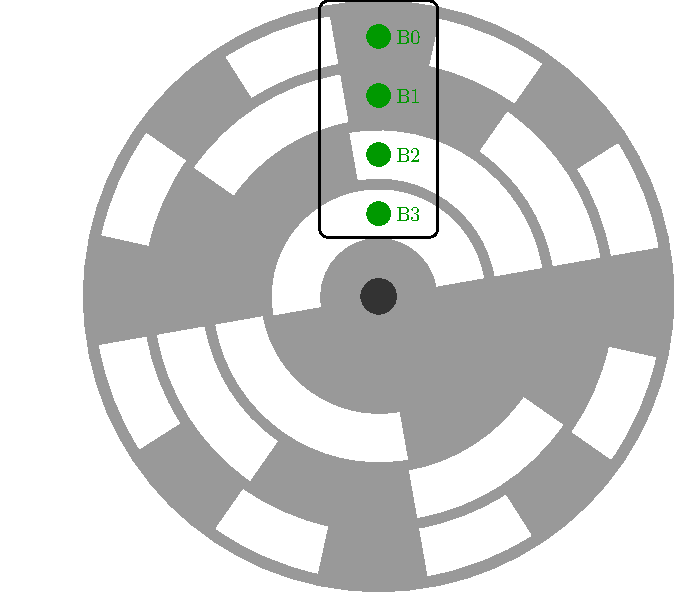
\includegraphics[width=0.35\textwidth]{../../figures/encoder-disc-absolute}\\
Encoder de cuatro bits.
\end{center}

Resolución requerida para el angula del brazo: \(\epsilon_b = 0.08^\circ\)


\alert{Actividad individual} Cual sería el número de bits necesario para un encoder absoluto montado directamente en el eje del brazo?
\end{block}
\end{frame}

\begin{frame}[label={sec:org648aafe}]{Posición del ala - Alternativ comercial 2}
\begin{center}
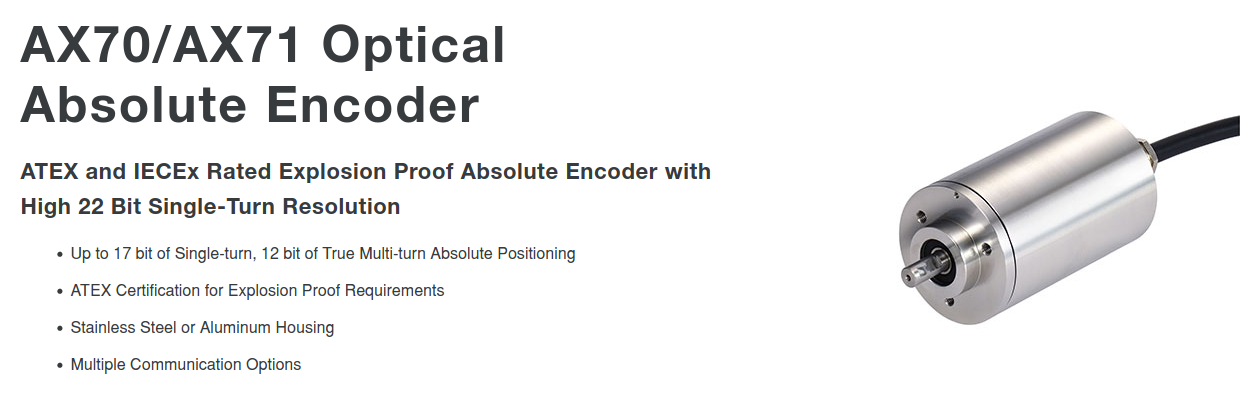
\includegraphics[width=0.99\linewidth]{../../figures/dynapar-absolute-encoder.png}\\
{\footnotesize Fuente: Dynapar.com}
\end{center}
\end{frame}
\end{document}